
\documentclass[12pt]{article}
\usepackage{amsmath}
\DeclareMathOperator*{\argmin}{arg\,min} % thin space, limits underneath in displays
\DeclareMathOperator*{\argmax}{arg\,max} % thin space, limits underneath in displays
\newtheorem{thm}{Theorem}
\usepackage{amssymb}
\usepackage{amsfonts}
\usepackage{mathrsfs}
\usepackage{bm}
\usepackage{indentfirst}
\setlength{\parindent}{0em}
\usepackage[margin=1in]{geometry}
\usepackage{graphicx}
\usepackage{setspace}
\doublespacing
\usepackage[flushleft]{threeparttable}
\usepackage{booktabs,caption}
\usepackage{float}
\usepackage{graphicx}
\usepackage[sort,comma]{natbib}
\usepackage[hidelinks]{hyperref}

\usepackage{import}
\usepackage{xifthen}
\usepackage{pdfpages}
\usepackage{transparent}

\newcommand{\incfig}[1]{%
\def\svgwidth{\columnwidth}
\import{./figures/}{#1.pdf_tex}
}



\usepackage{graphicx}
\usepackage{xspace,color}
\usepackage{url}
\usepackage{listings}


\lstset{commentstyle=\color{gray},keywordstyle=\color{black},
showstringspaces=false, basicstyle = \small
} %% basicstyle set fontsize
\lstnewenvironment{rc}[1][]{\lstset{language=R}}{}
\newcommand{\ri}[1]{\lstinline{#1}}  %% Short for 'R inline'



\lstdefinelanguage{language=R}{
numbers=left,
numberstyle=\footnotesize,
numbersep=1em,
xleftmargin=1em,
framextopmargin=2em,
framexbottommargin=2em,
showspaces=false,
showtabs=false,
showstringspaces=false,
frame=l,
tabsize=4,
}





\title{OLS}
\author{}
\date{}


\begin{document}
\maketitle


\section{Model}
\begin{equation*}
Y = \beta_0 + \beta_1 X_1 + \beta_2X_2 + ... + \beta_{p}X_{p} +
\varepsilon
\end{equation*}

You have $ n $ obs and $ p $ explanatory variables. For each obs, the
regression equation would be
\begin{equation*}
		y_{i} = \beta_0 + \beta_1x_{1,i} + \beta_2x_{2,i} + ... + 
		\beta_{p}x_{p,i} + \varepsilon_{i}
\end{equation*}
where $ i = 1,2,...,n $ stand for the $ i^{\text{ th }} $ obs.


{\textbf {Least-squared:}}
\begin{equation*}
\min_{\substack{\\}} \left( 
		\sum\limits_{i = 1} ^n(
		y_{i} - (\beta_0 + \beta_1x_{1,i} + \beta_2x_{2,i} + ... + 
		\beta_{p}x_{p,i})
		)	^{2}
\right)  
\end{equation*}


{\textbf {Matrix Form:}}
\begin{equation*}
\bm{Y} = \bm{X}\cdot \bm{\beta} + \bm{\varepsilon}
\end{equation*}
where $ \bm{Y} $ and $ \bm{\varepsilon} $ are $ n  \times 1 $ matrices
\begin{equation*}
\bm{Y} = 
\begin{bmatrix}
y_1\\y_2\\ \vdots  \\y_{n}
\end{bmatrix}
\quad
\text{ and }
\quad
\bm{\varepsilon} = 
\begin{bmatrix}
\varepsilon_1\\\varepsilon_2\\ \vdots  \\\varepsilon_{n}
\end{bmatrix}
\end{equation*}


\begin{equation*}
\bm{\beta} = 
\begin{bmatrix}
\beta_0\\\beta_1\\ \vdots \\\beta_{p}
\end{bmatrix}
\quad
\text{ and }
\quad
\bm{X} = 
\begin{bmatrix}
1 & x_{1,1} &\cdots&x_{p,1}\\
1 & x_{1,2} &\cdots&x_{p,2}\\
\vdots & \vdots &\ddots &\vdots \\
1 & x_{1,3} &\cdots&x_{p,3}\\
\end{bmatrix}
\end{equation*}


Matrix $ \bm{X} $ is $ n  \times (p + 1) $ dimension.


The OLS estimator $  \widehat{\bm{\beta}} $ :
\begin{equation*}
 \widehat{\bm{\beta}} = 
 \begin{bmatrix}
  \widehat{\beta}_{0}\\  \widehat{\beta}_{1}\\ \vdots \\  
	\widehat{\beta}_{p}
 \end{bmatrix}
 = (\bm{X}^{T}\cdot \bm{X})^{ - 1}\cdot \bm{X}^{T}\cdot \bm{Y}
\end{equation*}

\noindent\fbox{%
\parbox{\textwidth}{%
Derivation:
\begin{align*}
\min \bm{e}'\bm{e} &= \min \bm{(y - X   \widehat{\beta})'(y - X   \widehat{\beta})}\\
&= \bm{y'y - y'X  \widehat{\beta} -  \widehat{\beta}' X'y +  \widehat{\beta}'X'X 
 \widehat{\beta} }
\end{align*}
Note, $ \bm{ y'X  \widehat{\beta}} $, and $ \bm{ \widehat{\beta}' X'y} $ are scaler.
So the transpose of $ \bm{ y'X  \widehat{\beta}} $ is itself.
Remember the derivative of matrix: $ \frac{\partial \bm{x}'b }{\partial \bm{x} }
= b$

\begin{align*}
\frac{\partial \bm{e'e} }{\partial  \bm{\widehat{\beta}} }&= 0  
 - \frac{\partial (\bm{ \widehat{\beta}'X'y })' }{\partial \bm{ \widehat{\beta} } }
  - \bm{X'y} + 2 \bm{X'X  \widehat{\beta}} = 0\\
&= - \frac{\partial (\bm{ \widehat{\beta}'X'y }) }{\partial \bm{ \widehat{\beta} } }
  - \bm{X'y} + 2 \bm{X'X  \widehat{\beta}} = 0\\
&=  - \bm{X'y} - \bm{X'y} + 2\bm{X'X  \widehat{\beta}} = 0\\
2 \bm{X'X  \widehat{\beta}} &= 2 \bm{X'y}\\
\bm{ \widehat{\beta}}&= \bm{(X'X)^{ - 1}X'y}
\end{align*}
}%
}\\






\begin{figure}[H]
\center{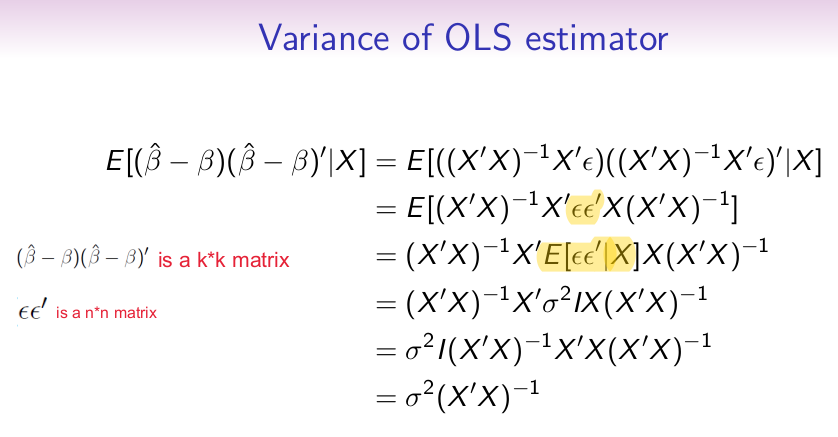
\includegraphics[scale =.6 ]  {figures/Variance_beta.png}}
\end{figure}



\begin{figure}[H]
\center{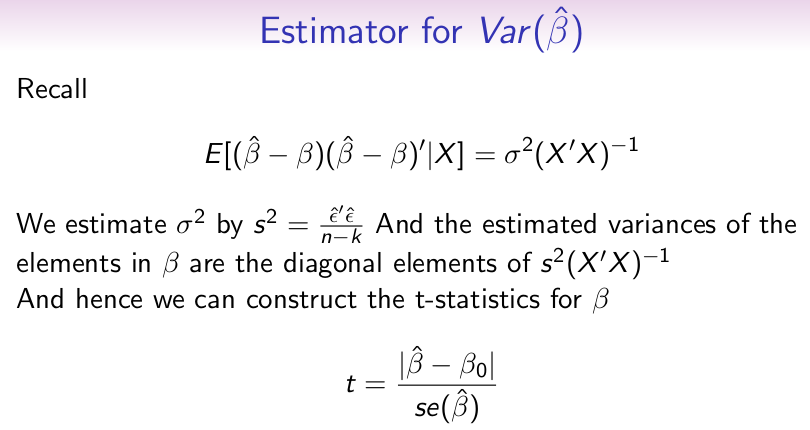
\includegraphics[scale =.6 ]  {figures/estimate_of_sigma2.png}}
\end{figure}



\begin{figure}[H]
\center{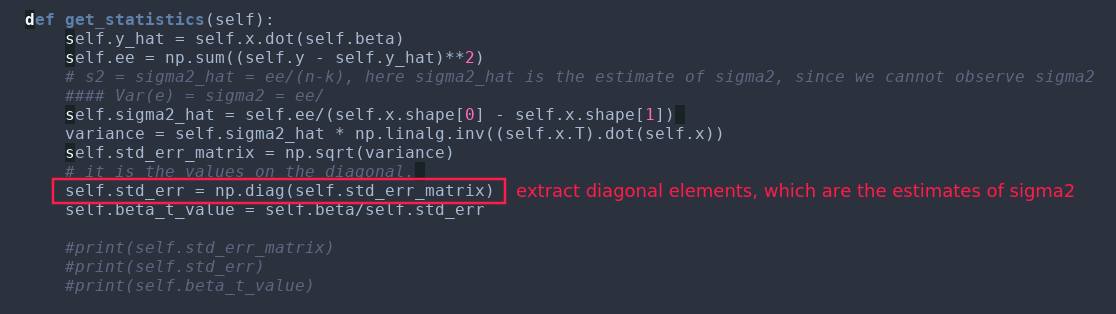
\includegraphics[scale =.45 ]  {figures/Variance_beta_code.png}}
\end{figure}










\subsection{F-test}
For a regression below:
\begin{equation*}
y = \beta_0 + \beta_1x_1 + \beta_2x_2 + ... + \beta_{k}x_{k} + \varepsilon
\end{equation*}
we usually want to know the significance of the regression equation, i.e., whether
all $ \beta $s equal to zero.
So we need to do a  $ F $-test with null below:
\begin{equation*}
H_0: \beta_1 = ... = \beta_{k} = 0
\end{equation*}
This null hypothesis can be written in this way:
\begin{equation*}
H_0: \beta_1 = 0, \beta_2 = 0, ... \beta_{k} = 0
\end{equation*}

Write this into vector form:
\begin{equation*}
H_0:
\begin{pmatrix}
		1 & 0 & 0\\
		0 & 1 & 0\\
		0 & 0 & 1\\
\end{pmatrix}
\begin{pmatrix}
\beta_1\\
\beta_2\\
\beta_3\\
\end{pmatrix}
=
\begin{pmatrix}
0\\
0\\
0\\
\end{pmatrix}
\end{equation*}
Let 
\begin{equation*}
\bm{R}= 
\begin{pmatrix}
		1 & 0 & 0 & \cdots &0\\
		0 & 1 & 0 & \cdots &0\\
		0 & 0 & 1 & \cdots &0\\
		\cdots&\cdots&\cdots&\cdots &\cdots\\
		0 & 0 & 0 & \cdots &1\\
\end{pmatrix},
\bm{\beta}= 
\begin{pmatrix}
\beta_1\\
\beta_2\\
\beta_3\\
\cdots\\
\beta_{k}
\end{pmatrix}
\bm{r}= 
\begin{pmatrix}
0\\
0\\
0\\
\cdots\\
0
\end{pmatrix}
\end{equation*}

$ \bm{R}: K  \times K, \quad \bm{\beta}: K  \times 1, \quad \bm{r}: m  \times 1$ 
In this case m = K

So, the null can be written in this way,
\begin{equation*}
H_0: \bm{R} \bm{\beta} - \bm{r} = 0
\end{equation*}
We can use quadratic form representing the distance between it and 0 and do the Wald
test
\begin{equation*}
		\frac{(\bm{R} \bm{\beta - r}  - 0)^{2}}{Var(\bm{R \beta - r})} = 
		(\bm{R  \widehat{\beta} - r})'[Var(\bm{R  \widehat{\beta} - r})]^{ - 1}
		(\bm{R  \widehat{\beta} - r})'
\end{equation*}
Form the $ F $ statistics:
\begin{equation*}
F = \frac{
		[(\bm{R  \widehat{\beta} - r})'[Var(\bm{R  \widehat{\beta} - r})]^{ - 1}
		(\bm{R  \widehat{\beta} - r})']/m
}{s^{2}} \sim F(m,n - K)
\end{equation*}


Note, 
\begin{align*}
		Var(\bm{R  \widehat{\beta} - r})&= Var(\bm{R  \widehat{\beta}})\\
		&= \bm{R}Var( \widehat{\beta})\bm{R}'\\
		&= \sigma^{2}\bm{R}(\bm{X'X})^{ - 1}\bm{R}'
\end{align*}
We use $ s^{2} $ to estimate $ \sigma^{2} $.

If $ F $ is very large, p value would be small. If p value is smaller than $ \alpha $,
reject the null.

{\textbf {We can also use $ F $-test to test if two estimators are equal.}}\\

Example:

For model: $ y = \beta_1 + \beta_2x_2 + \beta_3x_3 + \beta_4x_4 + \varepsilon $,
if you want to test:
\begin{equation*}
H_0: \beta_2 = \beta_3, \beta_4 = 0
\end{equation*}
it can be written as
\begin{equation*}
H_0: \beta_2 - \beta_3 = 0, \quad \beta_4 = 0
\end{equation*}
\begin{equation*}
H_0:
\begin{pmatrix}
\beta_2 - \beta_3\\
\beta_4
\end{pmatrix}
=
\begin{pmatrix}
0\\
0
\end{pmatrix}
\end{equation*}
\begin{equation*}
H_0:
\begin{pmatrix}
0 & 1 &  -1 & 0\\
0 & 0 &  0 & 1
\end{pmatrix}
\begin{pmatrix}
\beta_1\\
\beta_2\\
\beta_3\\
\beta_4\\
\end{pmatrix}
=
\begin{pmatrix}
0\\
0
\end{pmatrix}
\end{equation*}
\begin{equation*}
\bm{R} = 
\begin{pmatrix}
0 & 1 &  -1 & 0\\
0 & 0 &  0 & 1
\end{pmatrix}
, \quad
\bm{\beta} = 
\begin{pmatrix}
\beta_1\\
\beta_2\\
\beta_3\\
\beta_4\\
\end{pmatrix}
, \quad
\bm{r} = 
\begin{pmatrix}
0\\
0
\end{pmatrix}
\end{equation*}


\begin{equation*}
F = \frac{
		[(\bm{R  \widehat{\beta} - r})'[Var(\bm{R  \widehat{\beta} - r})]^{ - 1}
		(\bm{R  \widehat{\beta} - r})']/m
}{s^{2}} 
\end{equation*}
where $ s^{2} $ can be obtained in R using:
\begin{figure}[H]
\center{
\includegraphics[scale = ]  {figures/s2_from_R.png}}
\end{figure}



\subsection{Large vs small sample hypothesis testing}
In large sample case, we use asymptotic variance.


\subsubsection{t test for a single estimator}
In large sample case, $  \widehat{\beta} $ is asymptotically normal 
\begin{equation*}
		\sqrt {n}(\bm{ \widehat{\beta} - \beta}) \xrightarrow{d}N(\bm{0}, Avar(\bm{ \widehat{\beta}}))
\end{equation*}
For a specific $ \beta_{k} $,
\begin{equation*}
\sqrt {n}( \widehat{\beta}_{k} - \beta_{k}) \xrightarrow{d}N(0, Avar( \widehat{\beta}
_{k}))
\end{equation*}

\begin{equation*}
H_0:  \widehat{\beta}_{k} = c
\end{equation*}
\begin{equation*}
t_{k} = \frac{\sqrt {n}( \widehat{\beta}_{k} - c)}{
 \sqrt {\widehat{Avar( \widehat{\beta}_{k})}}
		} = 
\frac{ \widehat{\beta}_{k} - c}{
\sqrt {\frac{1}{n}\widehat{Avar( \widehat{\beta}_{k})}}
}=
\frac{ \widehat{\beta}_{k} - c}{
SE( \widehat{\beta}_{k})
}\xrightarrow{d} N(0,1)
\end{equation*}


{\textbf {Note: Now, t statistics follows asymptotic Normal distribution rather than t 
distribution. Statistics $ t_{k} $ is called robust $ t $ ratio}}


\subsubsection{F test}
In small sample, F statistics follows F distribution. In large sample, F statistics 
becomes $ W $ which follows Chi-square distribution, even though Stata still report F.

\begin{equation*}
		W = n(\bm{R  \widehat{\beta} - r})'[\bm{R} \widehat{Avar( \widehat{\beta})}\bm{R}']
^{ - 1}(\bm{R  \widehat{\beta} - r}) \xrightarrow{d} \chi^{2}(m)
\end{equation*}





\subsection{When to use robust std err}
If you believe there exist a conditional heteroskedasticity, use robust std err rather
than regular std err.
The coef in these two cases are same but std are different. Use regular std err under 
heteroskedasticity, you will largely under estimate the std err!!





\section{Heteroskedasticity}


\begin{enumerate}
\item 
OLS estimator is still unbiased, consistent and asymptotically normal under
heteroskedasticity.
\item 
The variance of OLS estimator, $ Var( \widehat{\bm{\beta}}|\bm{X}) $, is not
$ \sigma^{2}\bm{I} $. Hence we CANNOT implement $ t $ test and $ F $ test using 
regular standard error.
\item 
Gauss-Markov theorem no longer hold. OLS estimator is not BLUE.
\end{enumerate}

\subsection{Test Heteroskedasticity}
\begin{enumerate}
\item Draw residual plot. Vertical axis: residual, Horizontal axis: any explanatory
		variable ($ X_{i} $) or fitted value ($  \widehat{y} $).
\item Run BP test (Breusch and Pagan, 1979). BP test does not contain higher order
		terms in the conditional variance function.
\item Run While test (White, 1980). White test contains higher order terms in the
		conditional variance function.
\end{enumerate}


\subsubsection{BP test}
\begin{equation*}
y_{i} = \beta_0 + \beta_1x_{i 1} + \beta_2x_{i 2} + \cdots + \beta_{K}x_{i K} + \varepsilon_{i},
\end{equation*}
{\textbf {where $ i $ is the $ i $th observation}}.

Let $ \bm{x_{i}} = 
\begin{pmatrix}
1 &x_{i 1} &x_{i 2} &\cdots &x_{i K}
\end{pmatrix}
 $.
 Suppose the data are iid, then $ Var(\varepsilon_{i}|\bm{X}) = Var(\varepsilon_{i}
 | \bm{x_{i}})$.
 Therefore, the null hypothesis would be 
 \begin{equation*}
 H_0: Var(\varepsilon_{i}| \bm{x_{i}}) = \sigma^{2}
 \end{equation*}
 If there is {\textbf {no heteroskedasticity}}, the null hold.
 The null can be written in this way:
 \begin{equation*}
 H_0: E(\varepsilon_{i}^{2}| \bm{x_{i}}) = \sigma^{2}
 \end{equation*}
 If the null is not held, then $ \varepsilon^{2} $ would be a function of $ \bm{x_{i}} $.
 We call this function {\textbf {conditional variance function}}.

 Now suppose the conditional variance function is linear,
 \begin{equation*}
 \varepsilon_{i}^{2} = \delta_0 + \delta_1x_{i 1} + \cdots  + \delta_{i K} + u_{i}
 \end{equation*}
 Since we cannot observe $ \varepsilon $ directly, we need to use $ e^{2} $, and run
 the auxiliary regression below.
 \begin{equation*}
 e_{i}^{2} = \delta_0 + \delta_1x_{i 1} + \cdots  + \delta_{i K} +  error_{i}
 \end{equation*}

 If there's no heteroskedasticity, all $ \delta $s should be zero. Therefore we can 
 further rewrite the null hypothesis in this way:
 \begin{equation*}
 H_0: \delta_1 = \delta_2 = \cdots = \delta_{K} = 0
 \end{equation*}
 Then we can run a $ F $ test or Lagrange Multiplier test (LM). There's a 
 heteroskedasticity if we can reject the null.

 LM statistics:
 \begin{equation*}
 LM	 = nR^{2} \xrightarrow{d} \chi^{2}(K - 1)
 \end{equation*}

 {\textbf {Note:}} $ LM $ test and $ F $ test are asymptotically same when we have
 large samples.

\subsubsection{White test}
The conditional variance function is being considered in a linear form in BP test.
White test includes all squared terms (including interaction terms) in the auxiliary
regression.
For a regression model:
\begin{equation*}
y_{i} = \beta_0 + \beta_1x_{i 1} + \beta_2x_{i 2} + \varepsilon_{i}
\end{equation*}
the auxiliary regression would be
\begin{equation*}
e_{i}^{2} = \delta_0 + \delta_1 x_{i 1} + \delta_2x_{i 2} + \delta_3x_{i_1}^{2} + 
\delta_4x_{i 2}^{2} + \delta_5x_{i 1}x_{i 2} + error_{i}
\end{equation*}
Advantages of White test:\\
It can test all kinds of heteroskedasticity, since quadratic function can closely 
approximate all smooth function according to Taylor expansion.

Disadvantages of White test:\\
If there are many explanatory variables, there would be lots of squared terms. Lose
more degree of freedom.






\subsection{How to deal with heteroskedasticity}
\begin{enumerate}
\item OLS + robust std err
\item WLS (weighted least square)
\item FWLS (feasible weighted least square)
\end{enumerate}

\subsubsection{OLS + robust std error}
Under heteroskedasticity, run OLS and use robust std error rather than regular std err.
By using robust std err, we can still use $ t $ test and $ F $ test.

{\textbf {But it is less efficient. WLS/FWLS is more efficient.}}







\bibliographystyle{plainnat}
\bibliography{my_bib}

\end{document}


